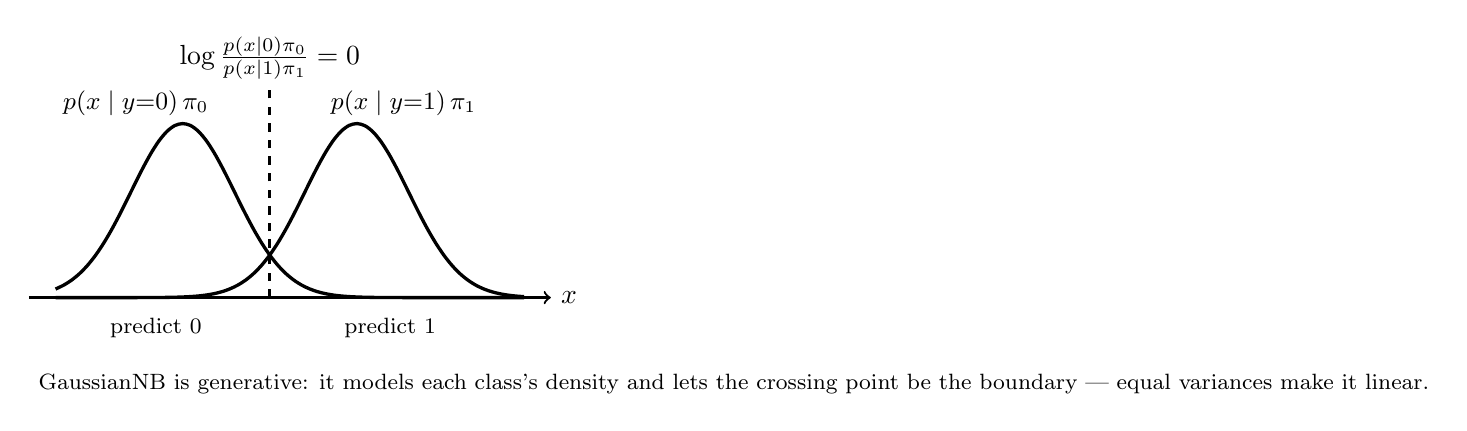
\begin{tikzpicture}[scale=0.85]
\draw[->, thick] (0,0) -- (7.8,0) node[right] {$x$};
% two class-conditional Gaussians, equal variance -> linear boundary
\draw[very thick, domain=0.4:7.4, smooth, samples=60]
  plot (\x, {2.6*exp(-((\x-2.3)^2)/1.2)});
\node[font=\small] at (1.6,2.9) {$p(x\mid y{=}0)\,\pi_0$};
\draw[very thick, domain=0.4:7.4, smooth, samples=60]
  plot (\x, {2.6*exp(-((\x-4.9)^2)/1.2)});
\node[font=\small] at (5.6,2.9) {$p(x\mid y{=}1)\,\pi_1$};
\draw[very thick, dashed] (3.6,0) -- (3.6,3.1)
  node[above] {$\log\frac{p(x|0)\pi_0}{p(x|1)\pi_1}=0$};
\node[font=\footnotesize] at (1.9,-0.45) {predict $0$};
\node[font=\footnotesize] at (5.4,-0.45) {predict $1$};
\node[align=left, anchor=north west] at (0,-1.0) {\footnotesize
  GaussianNB is generative: it models each class's density and lets
  the crossing point be the boundary --- equal variances make it
  linear.};
\end{tikzpicture}
